\documentclass[a4paper,11pt,notitlepage]{article}

\usepackage[english]{babel}
\usepackage[utf8x]{inputenc}
\usepackage[parfill]{parskip}
\usepackage{amsmath}
\usepackage{amssymb}
\usepackage{graphicx}
\usepackage{listings}
\usepackage[colorlinks=true]{hyperref}
\usepackage{algorithm}
\usepackage{algorithmicx}
\usepackage{algpseudocode}
\usepackage{enumitem}
\usepackage{tikz}

\lstset{
  language=Java,
  basicstyle=\footnotesize\ttfamily,
  numbers=left,
  breaklines=true,
  frame=lr,
  captionpos=b,
  showstringspaces=false,
  escapeinside={@*}{*@}
}
\newcounter{counter}

\title{ID1020 Project 1}
\author{Emil Tullstedt}

\hyphenation{definition algo-rithm}

\begin{document}
\maketitle

\tableofcontents

\newpage

\section{The Index}
\label{sec:theindex}

The implementation of the index constists of three different object types, where every word is stored within an \texttt{ArrayList} as an \texttt{EntryNode} within the \texttt{Dictionary} which in turn stores every document it occurs in within an \texttt{ArrayList} of \texttt{EntryData} which in turn has an ArrayList containing every occurrence.

Whenever something is added to \textit{either} of these lists, it is added using a BinarySearch-based insertion which ensures everything is sorted. This is done using the \texttt{getOrInsert}-method within the \texttt{BinarySearch}-class, which has the property that it also ignores any further occurrances of an element.

Essentially, this means that our \texttt{getOrInsert} can guarantee three things:

\begin{enumerate}
\item All elements are in order
\item There are not multiple occurrances of any single element
\item The words are inserted in a maximum $O(\log n)$ time
\end{enumerate}

The result after running the driver which inserts every word within the dictionary and updates the attributes to add every occurrence to every document is that we have a list of every word and where they appear.

By utilizing a function within \texttt{Dictionary} to use the \texttt{BinarySearch}-search method, we can find any word in $\sim\log n$ time.

The relation between the different elements that makes up the index can be seen in figure \ref{fig:dictionary}.

\begin{figure}[h!]
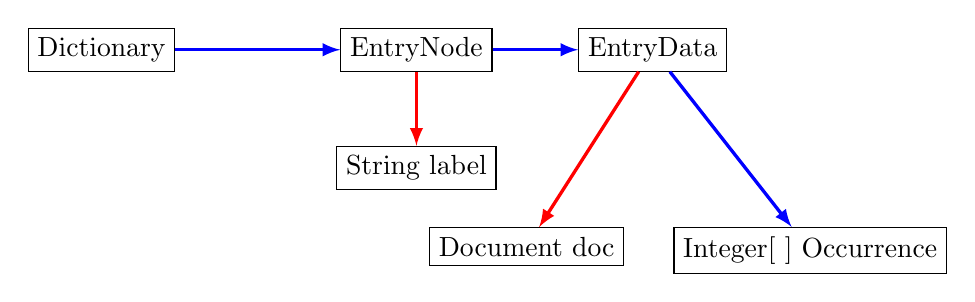
\begin{tikzpicture}
  \node[draw] (Dictionary) at (-4,0) {Dictionary};
  \node[draw] (EntryNode) at (0,0) {EntryNode};
  \node[draw] (Label) at (0, -1.5) {String label};
  \node[draw] (EntryData) at (3,0) {EntryData};
  \node[draw] (Document) at (1.4, -2.5) {Document doc};
  \node[draw] (Occurrence) at (5, -2.55) {Integer$[\ ]$ Occurrence};
  
  \draw[->,draw=blue, >=latex, very thick] (Dictionary) to (EntryNode);
  \draw[->,draw=blue, >=latex, very thick] (EntryNode) to (EntryData);
  \draw[->,draw=red, >=latex, very thick] (EntryNode) to (Label);
  \draw[->,draw=red, >=latex, very thick] (EntryData) to (Document);
  \draw[->,draw=blue, >=latex, very thick] (EntryData) to (Occurrence);
\end{tikzpicture}
\caption{The word dictionary structure}
\label{fig:dictionary}
\end{figure}

\newpage
\section{BinarySearch \textit{\&} Swap}
The \texttt{BinarySearch} class contains two static methods, the \texttt{search} and the \texttt{getOrInsert} methods. The usage of these are somewhat explained in section \ref{sec:theindex}. The implementation and the reasoning will be examined in this chapter.

\begin{algorithm}
\caption{BinarySearch}
\label{BinarySearch}
\begin{algorithmic}
\Function{Search}{key, array}
	\If {array.length = 0}
		\State \Return -1
	\Else
		\State high $\gets$ array.length
		\State low $\gets$ 0
	\EndIf
	
	\While{low $<$ high}
		\State mid $\gets$ low $+ \frac{\text{high} - \text{low}}{2}$
		
		\If{array[mid] $>$ key}
			\State high $\gets$ mid
		\ElsIf{array[mid] $<$ key}
			\State low $\gets$ mid $+ 1$
		\Else
			\State \Return mid
		\EndIf
	\EndWhile
	
	\State \Return $-$mid$-1$
\EndFunction
\end{algorithmic}
\end{algorithm}

Beginning with the \textsc{Search} operation as seen in algorithm \ref{BinarySearch}, we have a very simple implementation of binary search which returns either of three possible types of data:

\begin{enumerate}
\item Where the element is (for any positive integer returned)
\item Where the element should exist (for any negative integer returned)
\end{enumerate}

\textit{Notable} is how the return value when the element is not found is set to $-\text{mid}-1$. This is so that if you enter a word that should be placed on the zeroeth position, you'll not end up with a bug or a need to do a further examination in the code that uses the \textsc{Search} method. This is copied from the behaviour of Oracle's implementation of \href{http://docs.oracle.com/javase/7/docs/api/java/util/Arrays.html}{java.util.Array.BinarySearch}.\footnote{This implementation has a slight bug, where it may be off-by-one with the return value from the insertion point}

The binary search operation begins with the mid element of the original arrays and compares it to the search word, or the \textit{key}, and continues in a similar fashion on the subarrays depending of if the key was either smaller or larger than the value examined. The binary search operates on a list approximately sized to half of the previous examination in any subsequent comparison from the first one. Essentially this causes the complexity of the operation to be $\sim \log n$ following the reasoning in the equations \ref{eq:fractions} and the equivalent equation \ref{eq:logfractions}.

\begin{equation}\label{eq:fractions}
n \to \frac{n}{2} \to \frac{n}{4} \to \frac{n}{8} \to \cdots \to \frac{n}{n/2} \to \frac{n}{n}
\end{equation}

\begin{equation}\label{eq:logfractions}
\frac{n}{2^0} \to \frac{n}{2^1} \to \frac{n}{2^2} \to \frac{n}{2^3} \to \cdots \to \frac{n}{2^{\log_2({n/2})}} \to \frac{n}{2^{\log_2({n})}}
\end{equation}

We can safely ignore any negative values when simply searching, and are thus done with proving that we can reach any element in our list using only $O(\log n)$ iterations.

%\subsection{Insertion using BinarySearch}

%The insertion algorithm is supersimple

\end{document}